\documentclass[conference]{IEEEtran}

\usepackage{graphicx}
\usepackage{hyperref}
\usepackage{xspace}
\usepackage{listings}
\usepackage[usenames, dvipsnames]{color}
         

\graphicspath{{./img/}}

\hyphenation{op-tical net-works semi-conduc-tor}


\lstset{language=Python}

\definecolor{LightGray}{RGB}{250,250,250}

\lstdefinestyle{custompython}{
	captionpos=b,                    % sets the caption-position to bottom
	% frame=tb,
	xleftmargin=\parindent,
	language=Python,
	basicstyle=\footnotesize\ttfamily,
	keywordstyle=\bfseries\color{MidnightBlue},
	stringstyle=\color{PineGreen},
  	commentstyle=\color{Magenta},
  	backgroundcolor=\color{LightGray}
}


\newcommand{\tool}{Flask Dashboard\xspace}
\newcommand{\zee}{Zeeguu\xspace}
\newcommand{\git}{\texttt{git}\xspace}
\newcommand{\install}{{\small \texttt{pip install flask\_dashboard}}\xspace}
\newcommand{\activeUserCount}{two hundred\xspace}
\newcommand{\code}[1]{\texttt{#1}\xspace}
\newcommand{\perspective}[1]{{\small {\texttt{#1}}\xspace}}

\usepackage{fourier-orns}

\definecolor{myred}{RGB}{230, 20, 70}
\definecolor{mygreen}{RGB}{60, 180, 75}


\newcommand{\niceseparator}
	{
		\begin{center}
  		% $\ast$~$\ast$~$\ast$
  		% $\clubsuit$~$\clubsuit$~$\clubsuit$
  		\leafleft
		\end{center}
	}

% Endpoint Names 
%\newcommand{\epDecoration}[1]{{\small {\bf #1}}\xspace}
\newcommand{\epDecoration}[1]{\code{#1}}

\newcommand{\epTranslations}{{\color{myred} \epDecoration{api.get\_possible\_translations}}\xspace}
\newcommand{\epOutcome}{\epDecoration{api.report\_exercise\_outcome}}
\newcommand{\epFeedItems}{\epDecoration{api.get\_article\_difficulties}}



% Author Comments / Discussion

\definecolor{mlcolor}{RGB}{140, 140, 205}
\definecolor{vacolor}{RGB}{255, 0, 255}

\newcommand{\ml}[1]{ 
	{\footnotesize \color{mlcolor}ML: #1}
	}

\newcommand{\va}[1]{ 
	{\footnotesize \color{vacolor}VA: #1}
}


\newcommand{\mltp}[1]{\ml{Thijs, Patrick: #1}}
\newcommand{\mlv}[1]{\ml{Vasilios: #1}}

\definecolor{todocolor}{RGB}{200, 140, 160}

\newcommand{\todo}[1]{ 
	{\footnotesize \color{todocolor}Todo: #1}
	}

\newcommand{\Fref}[1]{Fig.~\ref{#1}}
\newcommand{\Sref}[1]{Sec.~\ref{#1}}




\begin{document}
%
\title{\tool: A Lightweight Analytics Platform for Visualizing Evolving Python Web Service Utilization and Performance}
% Alternative Titles: The Importance of Visualization in the Performance Monitoring of Python Web Services


% author names and affiliations
% use a multiple column layout for up to three different
% affiliations
%\author{\IEEEauthorblockN{Michael Shell}
%\IEEEauthorblockA{School of Electrical and\\Computer Engineering\\
%Georgia Institute of Technology\\
%Atlanta, Georgia 30332--0250\\
%Email: http://www.michaelshell.org/contact.html}
%\and
%\IEEEauthorblockN{Homer Simpson}
%\IEEEauthorblockA{Twentieth Century Fox\\
%Springfield, USA\\
%Email: homer@thesimpsons.com}
%\and
%\IEEEauthorblockN{James Kirk\\ and Montgomery Scott}
%\IEEEauthorblockA{Starfleet Academy\\
%San Francisco, California 96678--2391\\
%Telephone: (800) 555--1212\\
%Fax: (888) 555--1212}}

\author{
\IEEEauthorblockN{NAMES ORDER TBA}\\
Johann Bernoulli Institute for Mathematics and Computer Science\\
University of Groningen\\
Groningen, the Netherlands\\
Email: \{v.andrikopoulos,m.f.lungu\}@rug.nl, \{t.klooster.1,p.p.vogel\}@student.rug.nl
}

% make the title area
\maketitle

\begin{abstract}
The abstract goes here.
\end{abstract}

% no keywords

\IEEEpeerreviewmaketitle



\section{Introduction}

%Every system is a distributed system nowadays \cite{cavage2013there}. Indeed a very large number of applications and web applications are nowadays implemented as two-tier architectures with a front-end implemented with web technologies and a service back-end.
%\ml{I'm not completely happy with this paragraph}
``There is no getting around it: you are building a distributed system'' argues a paper from half a decade ago \cite{cavage2013there}. Indeed even the simplest student project web application ends up implemented as two-tier architectures with a front-end implemented with web technologies and a service backend usually a REST API.

% \hfill mds
Many contemporary programming languages are offering libraries, modules, or frameworks that facilitate the development of such architectures. Python is an example of such a language. 
% \hfill August 26, 2015
%
Python is currently one of the most popular programming languages for service implementation on the back-end side of web applications\footnote{Searching for projects written in Python on GitHub returns more than 500K open source projects as results}. At the time of writing this paper\footnote{End of June 2017} Python is the 4th most popular programming language according to the Tiobe Index\footnote{TIOBE programming community index is a measure of popularity of programming languages, created and maintained by the TIOBE Company based in Eindhoven, the Netherlands}. 
 
% possible flask summary
Flask\footnote{\url{http://flask.pocoo.org/}} is a very popular Python web framework\footnote{More than 25K projects on GitHub (5\% of all Python projects) are implemented with Flask (cf. a GitHub search for ``language:Python Flask'')}. It provides simplicity and flexibility by implementing a bare-minimum web server, and thus advertises as a micro-framework. The Flask tutorial shows how setting up a simple Flask ``Hello World'' web-service requires no more than 5 lines of Python code \cite{ flask:tutorial}.
% end of summary
 
To the best of our knowledge, however, there is no dedicated solution for monitoring the performance of Flask web applications. Thus, every one of those Flask projects faces one of the following options when confronted with the need of gathering insight into the runtime behavior of their implemented services: 

  \begin{enumerate}

    \item Use a commercial monitoring setup that usually requires setting up a different server that treats the subject API as a black-box (see \Sref{sec:related}). 

    \item Implement their own analytics toolchain potentially requiring multiple person-months. 

    \item Live without analytics insight into their services. \footnote{This is very real option: and is exactly what happened to the API that will be presented in this case study for many months. }

  \end{enumerate}

%\todo{For the first point in the list, we can also argue that analytics solutions like Google Analytics can be used, but they have no notion of versioning/integration with the development life cycle. Feel free to cite \cite{papazoglou2011managing} for service evolution purposes}

For projects which are done on a budget (e.g. research projects, startups) the first and the second options are often not available due to time and financial constraints. Furthermore, while adopting 3rd-party analytics solutions like e.g.~Google Analytics might be an option, a critical insight into the evolution of the exposed services of the web application, see for example~\cite{papazoglou2011managing}, is missing due to the fact such solutions have no notion of versioning/integration with the development life cycle.

To avoid such projects ending up in the third situation, in this paper we present a low-effort, lightweight service monitoring API for Flask-based Python web services that is easy to integrate and provides multiple perspectives on the performance and utilization of the subject API.
%\va{@all: I moved the remaining of this section to the Dashboard section since it makes more sense there} \ml{cool!}

\va{Mircea: consider removing the subsection header completely to save space}
  \subsection* {Structure of the Paper}
    
    \ml{to update!}
    The remainder of this paper is structured as follows: In Sections \ref{sec:util}, \ref{sec:perf}, \ref{sec:user} we dedicate a separate section to three types of analysis that \tool supports and present a the way the visualizations support these types of analysis. 



\section{Case Study}

  
  \zee\footnote{\url{https://www.zeeguu.unibe.ch/}} is a platform and an ecosystem of applications for accelerating vocabulary acquisition in a foreign language \cite{Lungu16}. 
%
  The architecture of the ecosystem has at its core an API implemented with Flask and Python and a series of satellite applications that together offer three main intertwined features for the learner:

  \begin{enumerate}

    \item Reader applications that provide effortless translations for those texts which are too difficult for the readers.

    \item Interactive exercises personally generated based on the preferences and past likes of the learner.

    \item Article recommendations which are at the appropriate level of difficulty for the reader. The difficulty is estimated based on past exercise and reading activity.

  \end{enumerate}

  The core API provides correspondingly three types of functionality: contextual translations, article recommendations, and personalized exercise suggestions. The core API of system is a research project, which sustains at the moment of writing this article the reading and practice of about \activeUserCount active beta-tester accounts. 

  In the remainder of this paper, we will use the \zee API as a case study. All the figures in this paper are captured from the actual deployment of \tool in the context of the \zee API \footnote{Within the \tool the figures are interactive offering basic data exploration capabilities: filter, zoom, and details on demand\cite{Shne99a}}.


% \ml{we should consider adding also one section in which the architecture/implementation and main features of the dashboard are presented before going on with discussing them in more depth in the following sections --- this should include a rundown on which views are provided from where (overview or per endpoint)}



\section{The \tool}

  The \tool as well as the web application that is being monitored in the case study is written in Python using Flask. This makes binding to the web services of the application relatively easy, as well as adding additional routes to the service for interacting with the \tool.

  To start using our Python library for service visualization, and assuming Flask is already installed, one needs to install the Python package\footnote{Section \ref{sec:install} shows how to install the package} 
  and simply add two lines of code to their Flask web service:

  % caption=Configuring the \tool is straightforward,
  \begin{lstlisting}[style=custompython]
  import dashboard
  ...
  # flask_app is the Flask app object
  dashboard.bind(flask_app)
  ...
  \end{lstlisting}


  % A custom route can also be defined by simply adding one extra line of code:
  % \begin{lstlisting}[caption=Configuring the \tool with a custom route for it to be accessed on is straightforward, style=custompython]
  % dashboard.config.link = 'custom-link'
  % \end{lstlisting}

  %\mltp{a small description of how the dashboard automatically intercepts the calls to the various API calls}
  After binding to the service, the \tool becomes available at the \texttt{/dashboard} route of the Flask application. A custom route can also be defined by the programmer in a configuration file.

  During binding, the \tool will search for all endpoints defined in the target application. These will be presented to the user in the tool web interface, where the user can select the ones that should be monitored, see \Fref{fig:sep}. 

    % \mltp{a small screenshot of how the dashboard allows one to select the interesting }
    \begin{figure}[h!]
      \centering
      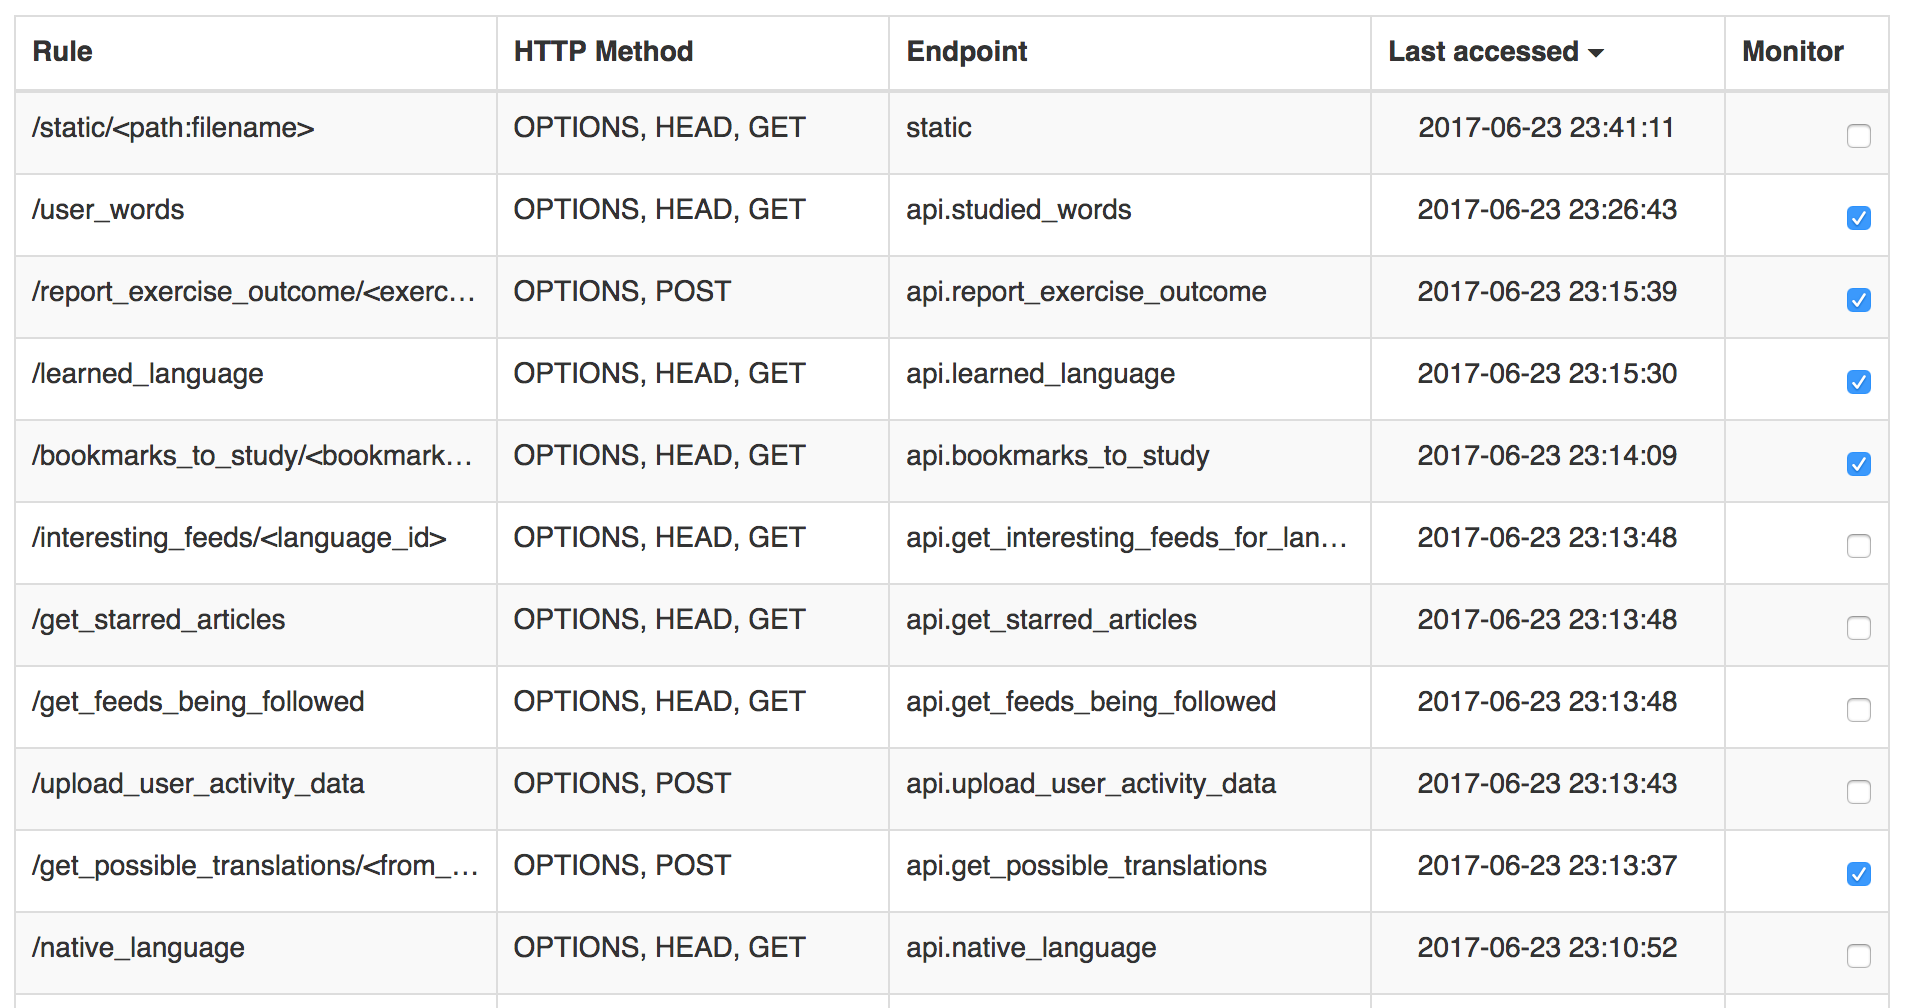
\includegraphics[width=\linewidth]{selecting_endpoints.png}
      \caption{All of the endpoints of the Zeeguu app are shown such that a selection can be made for monitoring them}
      \label{fig:sep}
    \end{figure}

  In order to monitor an endpoint, the \tool creates a function wrapper for the API function that corresponds to the endpoint. This way, the wrapper will be executed whenever that API call is made. The wrapper contains the code that takes care of monitoring an endpoint.
%
  \todo{Data collected by the wrappers are persisted in...}

  There are two main categories of visual perspectives that are available using \tool:
  \begin{enumerate}
    \item \textit{Overviews} that present information and measurements about all the endpoints of interest, and
    \item \textit{Detailed information} about the measurements pertaining to a specific endpoint.
  \end{enumerate}

  In the remainder of the paper we present several of these perspectives.\footnote{We recommend obtaining a color version of this paper for better readability}

  % The second endpoint conists of two parts, one of them being a table that shows for every monitored endpoint the number of hits it has gotten, the time it was last accessed and its average execution time. The second part is a view with four graphs which show:
  % \begin{itemize} 
  %   \item A heatmap of the total number of requests to the monitored endpoints
  %   \item A stacked bar chart that shows the total number of requests to the monitored endpoints per endpoint per day
  %   \item A boxplot graph showing the average execution time per version of the web service
  %   \item A boxplot graph showing the average execution time for every monitored endpoint
  % \end{itemize}


%!TEX root=vissoft.tex

\section{Service Utilization}
\label{sec:util}

  The most fundamental insight that a service maintainer needs regards service utilization. \vspace{0.5cm}

  Figure \ref{fig:aeu} shows a first perspective on endpoint utilization that \tool provides: a stacked bar chart of the number of hits to various endpoints grouped by day  shows that at its peak the API has about 2500 hits per day. 
  The way users interact with the platform can also be inferred since the endpoints are indicators of different activity types, e.g.: 

  \begin{enumerate}

    \item {\color{myblue}\epTranslations} is an indicator of the amount of foreign language reading the users are doing

    \item {\color{myviolet} \epOutcome} is an indicator of the amount of foreign vocabulary practice the users are doing

  \end{enumerate}


  \begin{figure}[!ht]
    \centering
    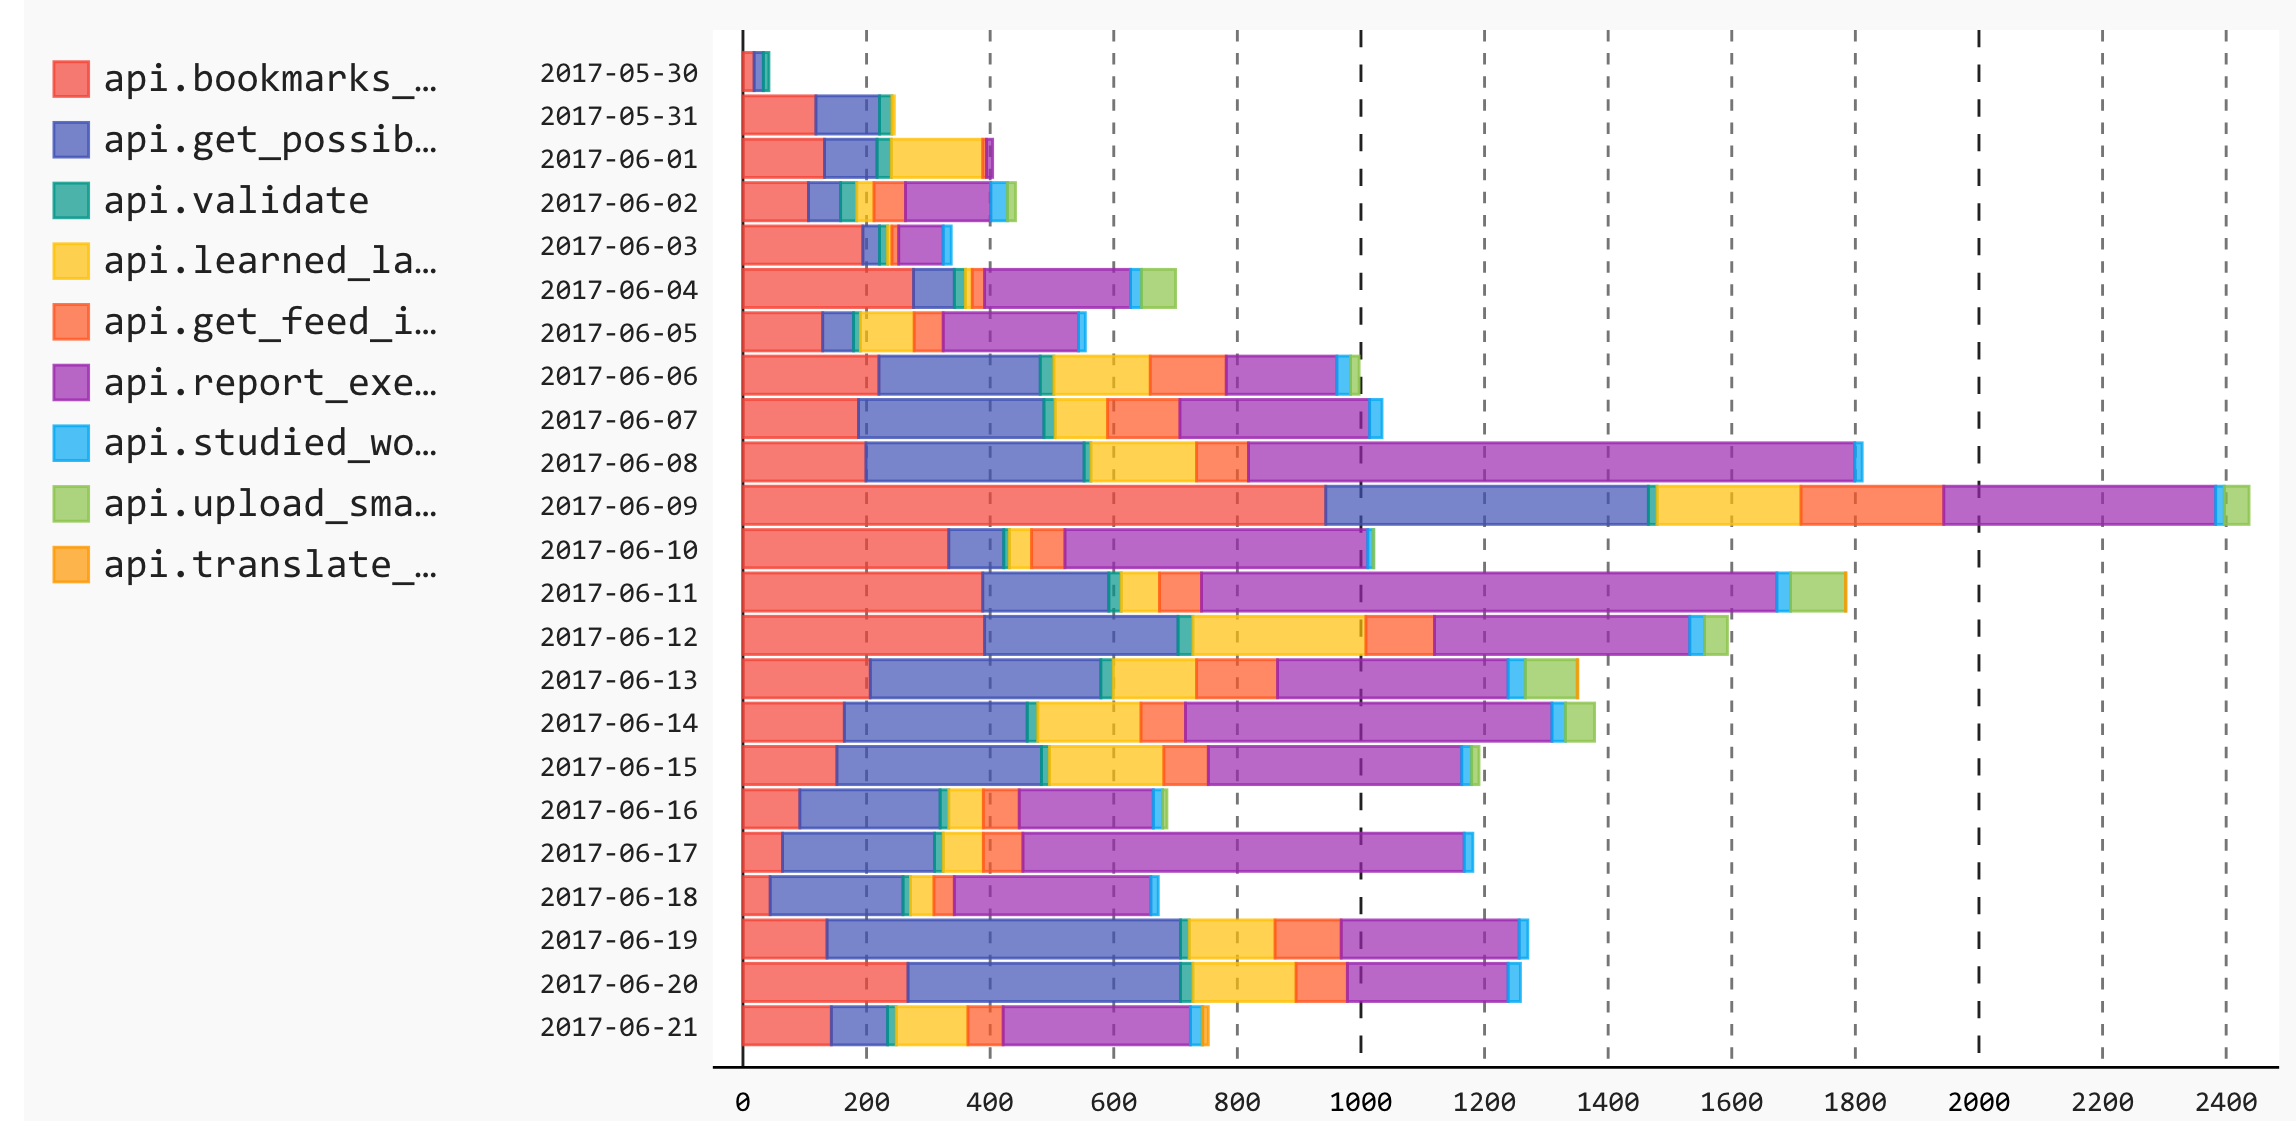
\includegraphics[width=\linewidth]{all_endpoints_usage.png}
    \caption{The number of requests per endpoint per day view shows the overall utilization of the monitored application}
    \label{fig:aeu}
  \end{figure}

  Besides showing the overall utilization, this endpoint provides to the maintainer with information relevant for decisions regarding endpoint deprecation -- one of the most elementary ways of {\em understanding the needs of the downstream}\cite{Haen14a}. In our case study, the maintainer realized that several endpoints which they thought were not being used, contrary to their expectations, were actually being used.\footnote{Usage information can also be used to increase the confidence of the maintainer that a given endpoint is not used, although it can never be used a proof.}

  \niceseparator

   \todo{Add the time series graph and discuss it before the heatmap? We can then sell the heatmap better} 
   \ml{Not sure about which graph you refer to here V}

  A second type of utilization question that the \tool can answer automatically regards {\em cyclic patterns of usage per hour of day}. 

  % \mltp{ can we add vertical lines that highlight the beginning of a new week (e.g. before Sunday): }
  % Patrick: adding separators in the graph is unfortunately not supported by the library.

    \begin{figure}[!ht]
      \centering
      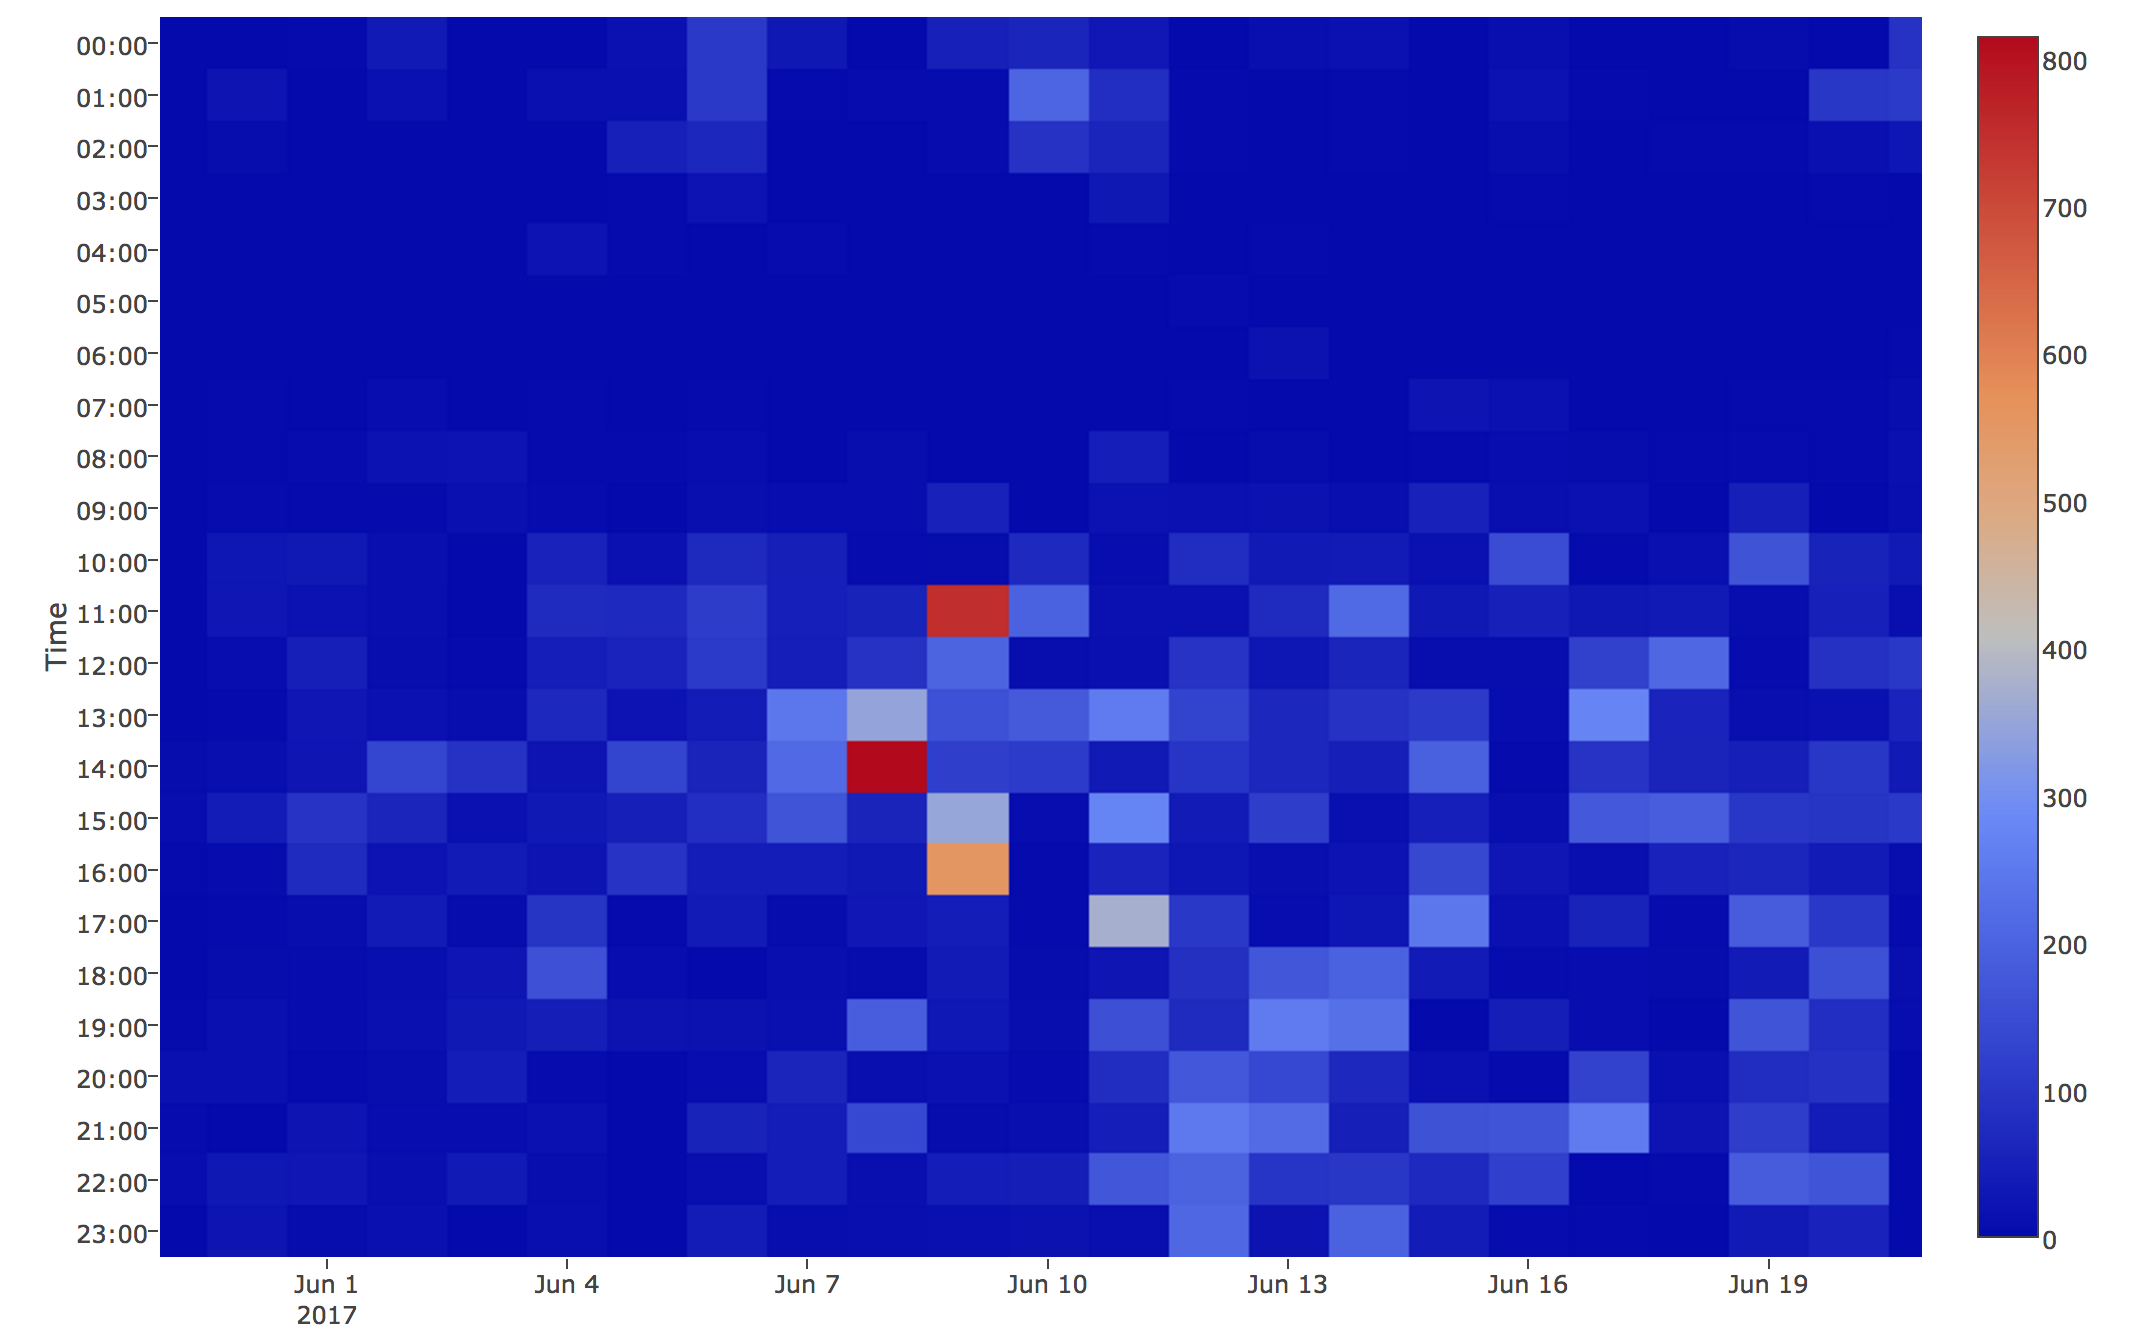
\includegraphics[width=\linewidth]{daily_patterns}
      \caption{Usage patterns become easy to spot in the requests per hour heatmap}
      \label{fig:dp}
    \end{figure}


  Figure \ref{fig:dp} shows the the API not being used during the early morning hours, and that most of the activity focused around working hours and some light activity during the evening. This is consistent with the fact that the current users are all in the central european timezone. 




\section{Endpoint Performance}
\label{sec:perf}

  The \tool also collects information regarding endpoint performance. The view in Figure \ref{fig:ep} summarizes the response times for various endpoints by using box-and-whisker plots. 

  % \ml{Thijs and Patrick... the visualization people will complain when they see that we have different colors for the same endpoint in different graphs. Can we insure that there is consistency in colors? Simplest trick would be to obtain the color by hashing the name of the endpoint... in that case the same endpoint would have the same color in various graphs.}
  % This is supported in the latest version of the dashboard

  \begin{figure}[!ht]
    \centering
    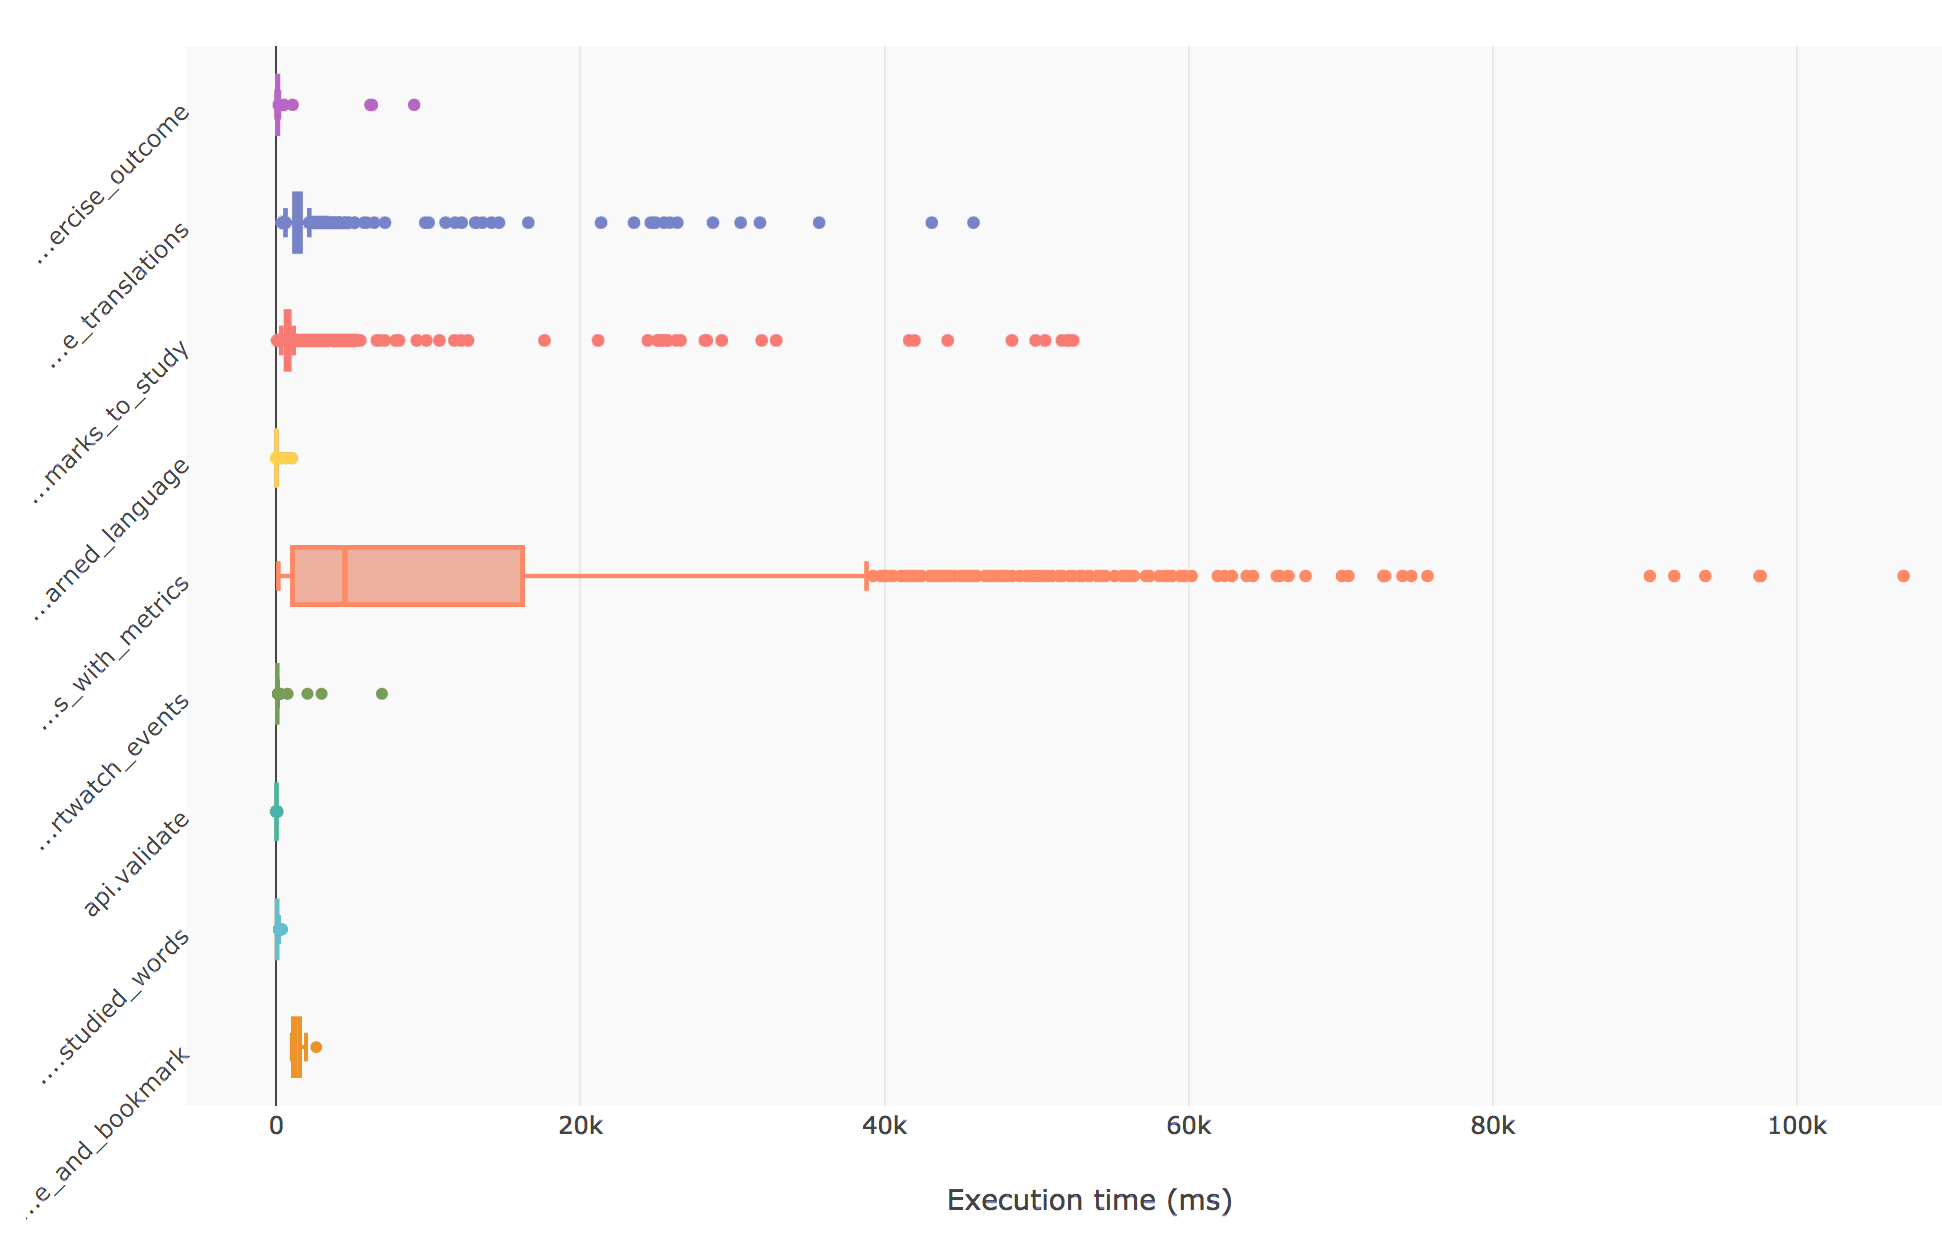
\includegraphics[width=\linewidth]{endpoint_performance.png}
    \caption{The response time (in ms) per monitored endpoint view allows for identifying performance variability and balancing issues}
    \label{fig:ep}
  \end{figure}

  After investigating this view it became clear to the maintainer that three of the endpoints had very large variation in performance. One of the three was most critical was optimized first: the \epTranslations is part of a live interaction and it having such variable performance was a usability problem for the users of the reader applications. 

  % most important endpoints that they decided to improve the performance of is the second from the top in Figure \ref{fig:ep}: the endpoint that returns translations. This is particularily critical since it is part of a live interaction loop. 


  \niceseparator

  To be able to see their improvements in action, the maintainer had to add an extra configuration information to be able to find the `.git' folder from where to retrieve the current version of the deployed application: 

  \begin{lstlisting}[caption=Configuring the \tool with the path to the .git folder enables the generation of evolutionary performance graphs, style=custompython]

dashboard.config.git = 'path/to/.git'


    \end{lstlisting}

  After redeploying the API, the dashboard can now automatically detect the current version of the project, and can group measurements by version. \tool can now generate the view in Figure \ref{fig:tee} where the performance of the give endpoint is tallied by version.

    \begin{figure}[h!]
      \centering
      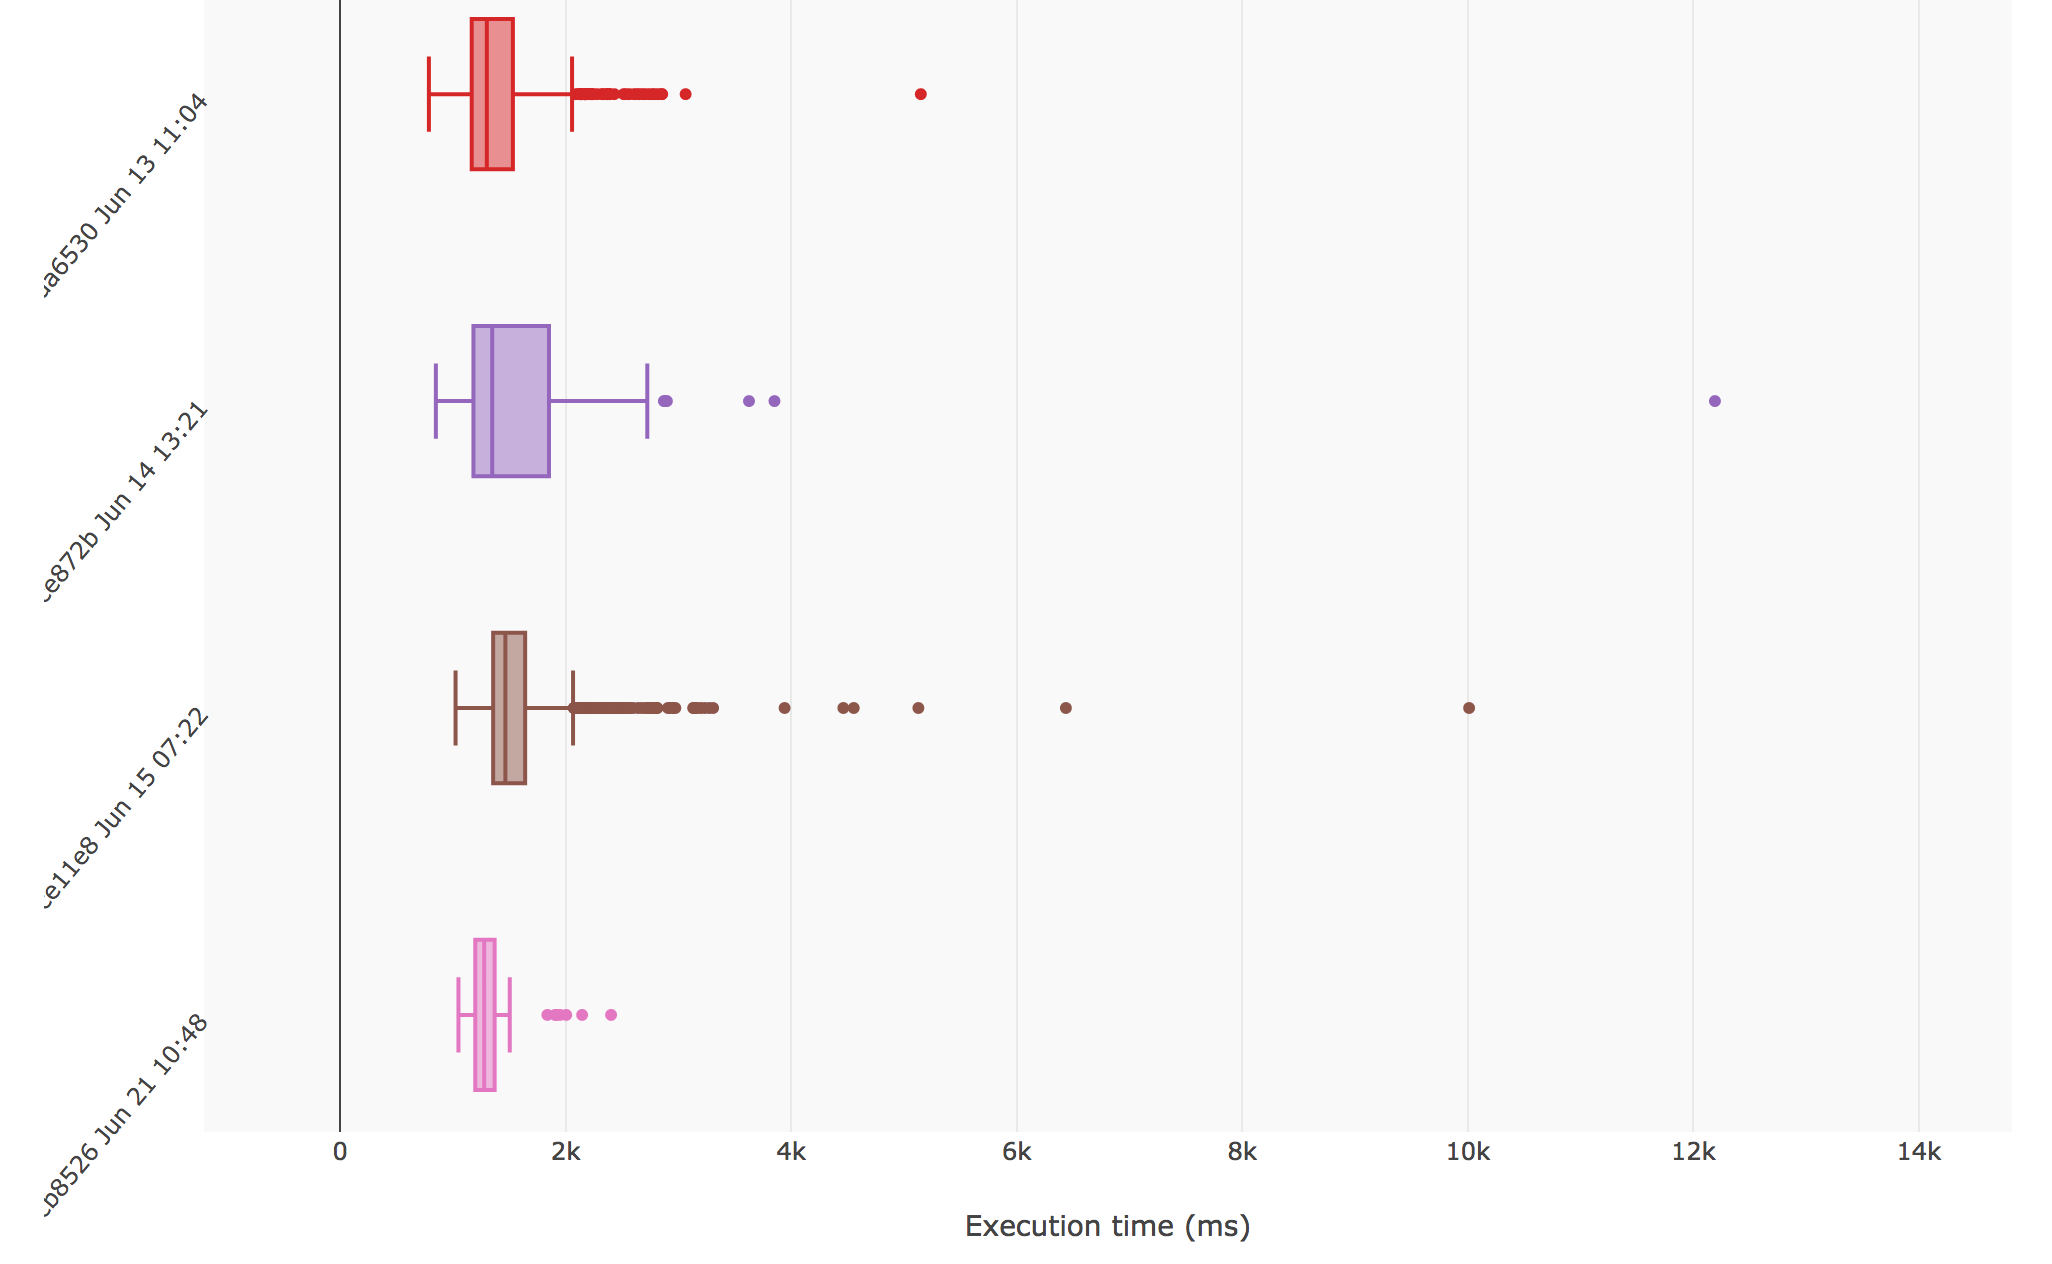
\includegraphics[width=\linewidth]{translation_endpoint_evolution.png}
      \caption{Visualizing The Performance Evolution of the \epTranslations endpoint}
      \label{fig:tee}
    \end{figure}

  This way the maintainer could confirm that the performance of the translation endpoint improved: in the latest version (bottom-most box plot in Figure \ref{fig:tee}) the entire box plot moved to the left and there are fewer outliers.


  \niceseparator

  The \tool also collects {\bf extra information about outliers}: Python stack trace, CPU load, request parameters, etc. in order to allow the maintainer to investigate the causes of these exceptionally slow response times. 

  In order to address this, but not degrade the usual performance the \tool tracks for every endpoint a running average value. When it detects that a given request is an outlier with respect to this past average running value, it triggers the {\em outlier data collection routine} which stores all the previously listed extra information about the current execution environment. 


\section {User Experience}
\label{sec:user}

  For service endpoints which run computations in real time, the operator of a system must understand the endpoint performance on a per-user basis, especially for situations where the system response time is a function of some individual user load\footnote{E.g. in GMail some users have two emails while other have twenty thousand and this induces different response times for different users}

  \tool provides a way of grouping information on a per user basis. However, to do this, the developer must specify the way in which a given API call can be associated with a given user. There are multiple ways, the simplest utilizes again the common expectations of Flask applications which offers a global \code{request} object which contains a \code{session} object which encapsulates information: 

  \begin{lstlisting}[float,caption=Simply define a custom app-specific function for user retrieval and pass it to the \tool to group information by user,style=custompython]
    
    # app specific way of extracting the user
    # from a flask request object    
    def get_user_id(request):
      sid = int(request.args['session'])
      session = User.find_for_session(sid)
      return user_id

    # attaching the get_user_id function
    dashboard.config.get_group_by = get_user_id

  \end{lstlisting}

  In the Zeeguu case study, one of the slowest endpoints, and one with the highest variability is \epFeedItems: it retrieves a list of recommended articles for a given user. However, since a user can be subscribed to anything from one to three dozen article sources, and since the computation of the difficulty is personalized and it is slow, the variability in time among users is likely to be very large. 


  Figure \ref{fig:tpu} shows some of the results of calling the \epFeedItems endpoint for various users. The figure shows that the response times for this endpoint can vary considerably for different users. 

  \begin{figure}[!ht]
    \centering
    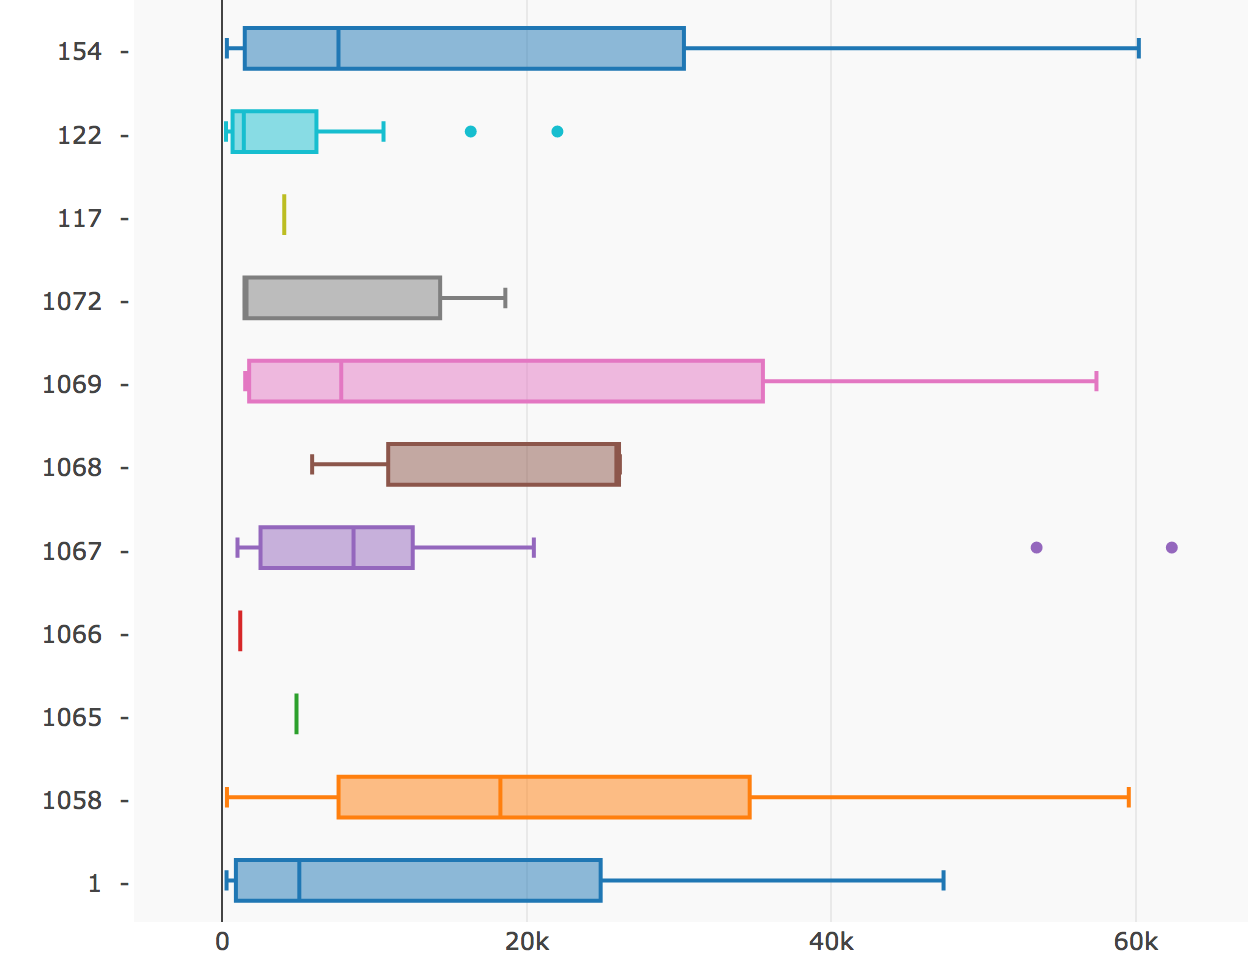
\includegraphics[width=\linewidth]{time_per_user}
    \caption{The \epFeedItems shows a very high variability across users}
    \label{fig:tpu}
  \end{figure}

  \niceseparator

  The limitation of the previous view is that it does not present the information also on a per version basis. To address this, a different visual perspective entitled \perspective{Evolving per-User Performance} can be defined. Figure \ref{fig:tuv} attempts to present the information that would be required in such an perspective: 

  \begin{figure}[!ht]
    \centering
    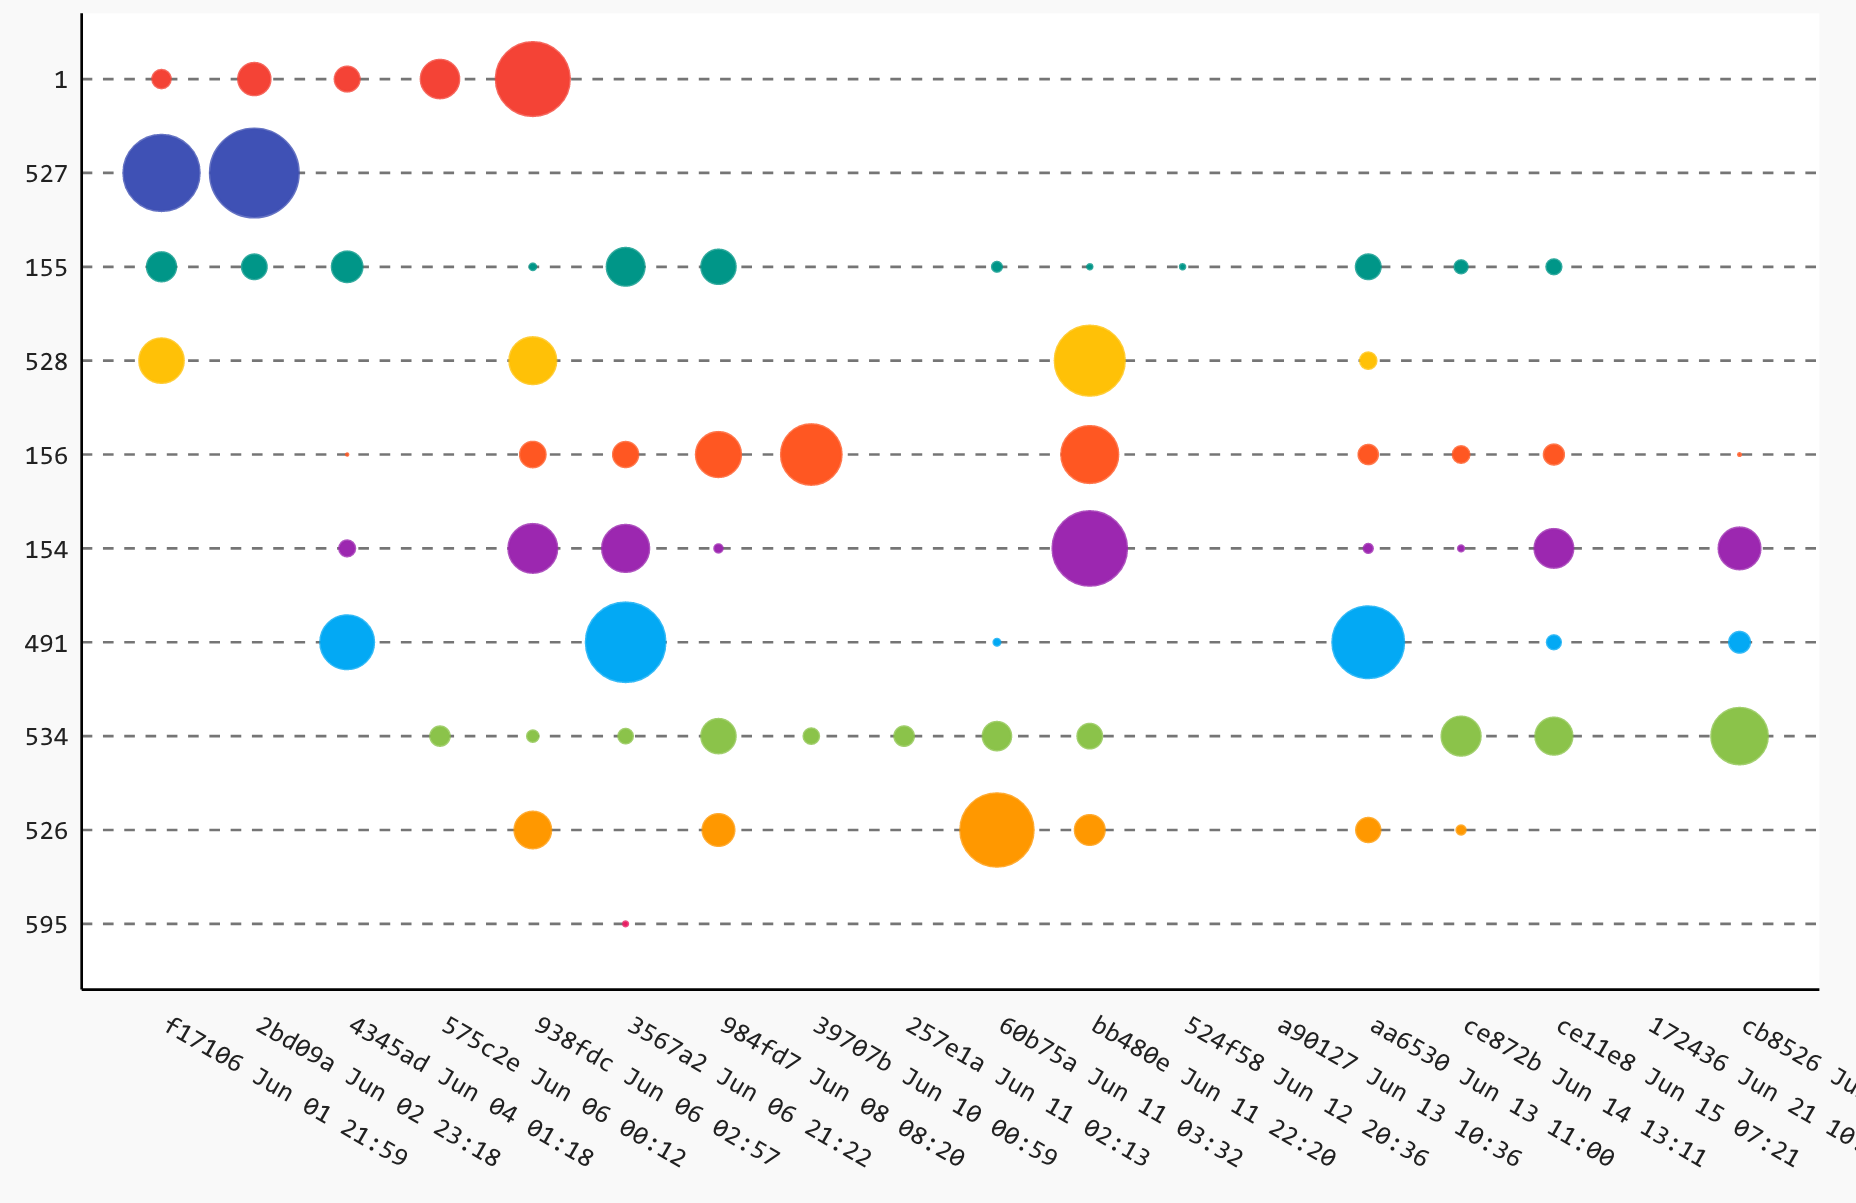
\includegraphics[width=\linewidth]{time_per_user_per_version}
    \caption{Caption here}
    \label{fig:tuv}
  \end{figure}

  For the situations in which the user information is not available, the \tool tracks out of the box information about different IPs. In some cases this might be a sufficiently good approximation of the user diversity and identity.

\section{Discussion}

  \subsection{Integrating with Different Deployment Strategies in Order to Automatically Monitor System Evolution}

  The main goal of the \tool design was to allow analytics to be collected and insight to be gleaned by making the smallest possible changes to the running API. To allow the collection of evolutionary information 

  This technique assumes that the web server code which is the target of the monitoring is deployed using \git in the following way: 

  \begin{enumerate}
    \item The deployment engineer pulls the latest version of the code from the integration server; this will result in a new commit being pointed at by the HEAD pointer than previously
    \item The deployment engineer restarts the new version of the service. At this point, the \tool detects that a new HEAD is present in the local code base and consequently starts associating all the new data points with this new commit\footnote{The \tool detects the current version of the analyzed system the first time it is attached to the application object, and thus, assumes that the Flask application is restarted when a new version is deployed. This is in tune with the current version of Flask, but if the web server will support dynamic updates in the future, this might have to be taken into account}
  \end{enumerate}

  The advantage of this approach is the need for minimal configurability. The disadvantage is that it will consider the smallest of the commits\footnote{Even one that modifies a comment} and the shortest lived commits\footnote{A commit which was active only for a half an hour before a new version with a bug fix was deployed}, as a distinct way of grouping the data points. 

  Another possible extension point here is supporting other version control systems (e.g. Mercurial). However, this is a straightforward extension.



  \subsection{User-Awareness }

    User awareness as presented in Section \ref{sec:user} is useful, but the scalability of the approach must be taken into consideration. In our case study we had about several hundreds users (of which about \activeUserCount were active during the ) 


  \subsection{Utilization}

    There are other perspectives on service utilization that could be useful, that we did not list in this paper. For example, if the service is using OAuth, then together with every request, in the header of the request there is information about the application which is sending a request. But providing statistics about 

  \subsection{Tool and Source Code Availability}
  \label{sec:install}

    \tool is implemented for Python 3.6 and is available on the Python Package Index repository\footnote{\url{http://pypi.org/TODO}} from where it can be installed on any system that has Python installed by running \install from the command line. 

    The code of \tool is published under a permissive MIT license and is available on GitHub.\footnote{\url{https://github.com/mircealungu/automatic-monitoring-dasboard}}

    The images in this paper are screenshots of the interactive visualizations from the deployment of \tool in the context of the Zeeguu core API. The actual deployment can be consulted online by the reviewers and readers of this article\footnote{\url{https://zeeguu.unibe.ch/api/dashboard}. Username: {\em guest}, password: {\em vissoft}}.


\section{Related Work}
\label{sec:related}

\ml{TODO}

Java Visualization \cite{Pauw02a}

Run-time monitoring of services \cite{ghezzi2007run}

An existing monitoring tool is Pingdom \footnote{https://www.pingdom.com/company/why-pingdom}, which monitors the uptime of an existing web-service. This tool works by pinging the websites (up to 60 times) every minute automatically. Thus this creates a lot of overhead and is bound to be noisy since it will also be influenced by the speed of the network connection\footnote{Another problem is that such a tool would }

\todo{Runscope? Others?}


\section{Conclusion and Future Work}

In this paper we have shown that it is possible to build a lightweight monitoring solution which provides plenty of feedback to a user with very little effort. 

In the future we plan to investigate ...
\ml{TODO}



% conference papers do not normally have an appendix


% use section* for acknowledgment
\section*{Acknowledgment}


The authors would like to thank...





% references section

\bibliographystyle{IEEEtran}
\bibliography{vissoft}


% that's all folks
\end{document}


